\documentclass[../main.tex]{subfiles}
\begin{document}
\section{Introduction}
\label{sec:intro}
\begin{figure}[H]
    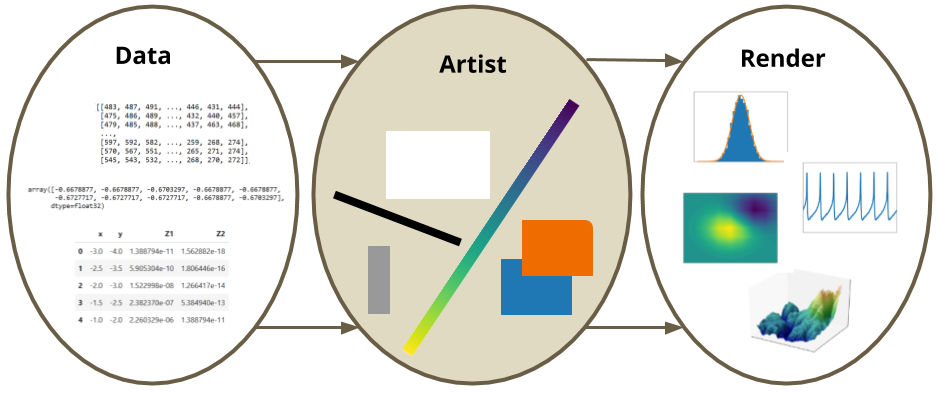
\includegraphics[width=\textwidth]{figures/math/dar.png}
    \caption{Visualization is equivariant maps between data and visual encoding of the variables and assembly of those encodings into a graphic.
    \note{will replace w/ overarching figure w/ same structure}}
    \label{fig:intro_artist_stages}
\end{figure}

 This work is motivated by a need for a visualization library that developers could build complex, domain specific tools tuned to the semantics and structure carried in domain specific data. The core architecture also needs to be robust to the big data needs of many visualization practitioners, and therefore support distributed and streaming data needs. To support both exploratory and confirmatory visualization\cite{tukeyWeNeedBoth1980}, this tool needs to support 2D and 3D,  static, dynamic and interactive visualizations. Specifically, this work was driven by a rearchiture the Python visualization library Matplotlib\cite{hunterMatplotlib2DGraphics2007} to meet modern data visualization needs. We aim to take advantage of developments in software design, data structures, and visualization to improve the consistency, composibility, and discoverability of the API. 

 This work presents a mathematical description of how data is transformed into graphic representations, as shown in figure~\ref{fig:intro_artist_stages}. While many researchers have identified and described important aspects of visualization, they have specialized in such different ways as to not provide a model general enough to natively support the full range of data and visualization types many general purpose modern visualization tools may need to support. In this work, we present a framework for understanding visualization as equivariant maps between topological spaces. Using this mathematical formalism, we can interpret and extend prior work and also develop new tools. We validate our model by using it to re-design artist and data access layer of Matplotlib, a general purpose visualization tool.
 

\section{Background}
Visual algorithms that display information are designed such that structure of data is assumed according to Tory and Möller  \cite{toryRethinkingVisualizationHighLevel2004}. Specifically they note that discrete and continuous data and their attributes form a discipline independent design space \cite{pousmanCasualInformation2007}. This idea can be seen in modern general purpose visualization architecture,  where many libraries are either defined around specific data structures or make implicit assumptions about the data or the types of visualizations they will support. In proposing a new architecture, we contrast the trade offs libraries make, describe different types of data continuity, and discuss metrics by which a visualization library is traditionally evaluated. 

\subsection{Tools}
\label{sec:intro_data_tools}
The library driving this rearchitecture, Matplotlib, aims to be flexible enough that developers can build domain specific libraries on top of it. To preserve this flexibility, Matplotlib enforces minimal constraints on what sorts of data the user is allowed to input and supports very many visual algorithms, from primative marks to computationally complex visualizations. Instead of enforcing constraints at the API level, Matplotlib carries implicit assumptions about data continuity in how each function interfaces with the input data. This has lead to poor API consistency and brittle code as every visual algorithm has a very different point of view on how the data is structured. 

A commonly cited alternative is the family of tools built on top of Wilkenson's Grammar of Graphics (GoG) \cite{wilkinsonGrammarGraphics2005}, including ggplot\cite{wickhamGgplot2ElegantGraphics2016a}, protovis\cite{bostockProtoviz2009} and D3 \cite{bostockDataDrivenDocuments2011}, vega\cite{satyanarayanDeclarativeInteractionDesign2014} and altair\cite{vanderplasAltairInteractiveStatistical2018}. This framework is very popular in the data visualization community their declarative interface \cite{heerDeclarative2010} which allows end users to describe the visualization they are trying to create. It is also the wrong abstraction layer since the grammer exposes specific ways to compose parts together to build a chart, but not ways to build new parts\cite{wongsuphasawatNavigatingWideWorld2021}.

A different class of user facing tools are those that support images, such as ImageJ\cite{schneiderNIHImageImageJ2012}. These tools mostly have some support for visualizing non image components of a complex data set, but mostly in service to the image being visualized. These tools are ill suited for general purpose library developers as the architecture is to build plugins into the existing system \cite{WritingPlugins} rather than domain specific tools that are built on top. Even the digital humanities oriented macro ImagePlot\cite{studiesCulturevisImageplot2021}, which supports some non-image aggregate reporting charts, is still built around image data as the primary input. 

There are also visualization tools designed around scientifically complex data that support explicit description of the data, such as vtk\cite{hanwellVisualizationToolkitVTK2015,geveci2012vtk} and its derivatives such as MayaVi\cite{ramachandranMayaVi2011} and extensions such as ParaView\cite{ahrens2005paraview}. These libraries, generally speaking, are architectured more as graphics libraries than visualization libraries, meaning they lack a clear distinction between the graphic construction and the rendering of that graphic. This is very close to the existing Matplotlib architecture, where the data, visual encoding, and rendering are jumbled in ways that make it hard to figure out what the code is doing. We are proposing a functional framework instead in large part to clearly encapsulate these separate responsibilities of a visualization tool. In turn, this should make it easier to reuse components in the building of new tools. 

\subsection{Data}
\label{sec:intro_data}
In this work, we extend Butler's topology driven representation of visualization data \cite{butlerVisualizationModelBased1989,butlerVectorBundleClassesForm1992}. Butler proposes that fiber bundles are a good model for visualization data because it allows for encoding the continuity of the data separately from the types of variables in the data. Fiber bundles are flexible enough to support discrete and ND continuous datasets. Since Butler's model lacks a robust way of describing the variables, we fold in Spivak's Simplacial formulation of databases \cite{spivakDatabasesAreCategories2010,spivakSIMPLICIALDATABASES} so that we can encode a schema like description of the data in the fiber bundle.

\begin{figure}[H]
    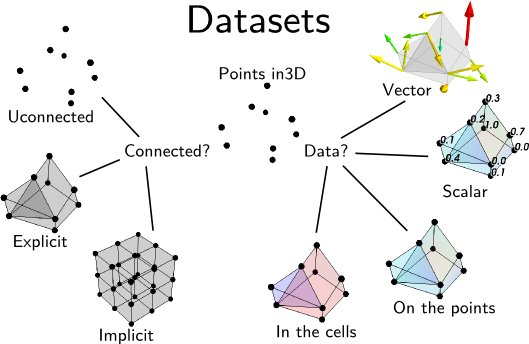
\includegraphics[width=1\textwidth]{figures/intro/dataset_diagram.png}
    \caption{One way to describe data is by the connectivity of the points in the dataset. A database for example is often discrete unconnected points, while an image is an implicitely connected 2D grid. This image is from the Data Representation chapter of the MayaVi 4.7.2 documentation.\cite{DataRepresentationMayavi}}
    \label{fig:intro_data_format}
\end{figure}
As shown in figure~\ref{fig:intro_data_format}, there are many types of connectivity. A database typically consists of unconnected records, while an image is an implicit 2D grid and a network is some sort of explicitly connected graph.  In this work we will refer to the points of the dataset as \textit{records} to indicate that a point can be a vector of heterogenous elements. Each \textit{component} of the record is a single object, such as a temperature measurement, a color value, or an image. We also generalize \textit{component} to mean all objects in the dataset of a given type, such as all temperatures or colors or images. The way in which these records are connected is the \textit{connectivity}, \textit{continuity}, or more generally \textit{topology}.

\begin{mdframed}[roundcorner=10pt, frametitle= definitions, frametitlerule=true, frametitlebackgroundcolor=gray!10]
\begin{definition}
    \item[records] points, observations, entries 
    \item[components] variables, attributes, fields 
    \item[connectivity] how the records are connected to each other
\end{definition}
\end{mdframed}

Often this topology has metadata associated with it, describing for example when or where the measurement was taken. Building on the idea of metadata as \textit{keys} and their associated \textit{value} proposed by Munzner \cite{munznerChDataAbstraction}, we propose that information rich metadata are part of the components and instead the values are keyed on coordinate free structural ids. In contrast to Munzner's model where the semantic meaning of the key is tightly coupled to the position of the value in the dataset, our model allows for renaming all the metadata, for example changing the coordinate systems or time resolution, without imposing new semantics on the underlying structure.

\subsection{Visualization}

\begin{figure}[H]
    \begin{subfigure}{.24\textwidth}
        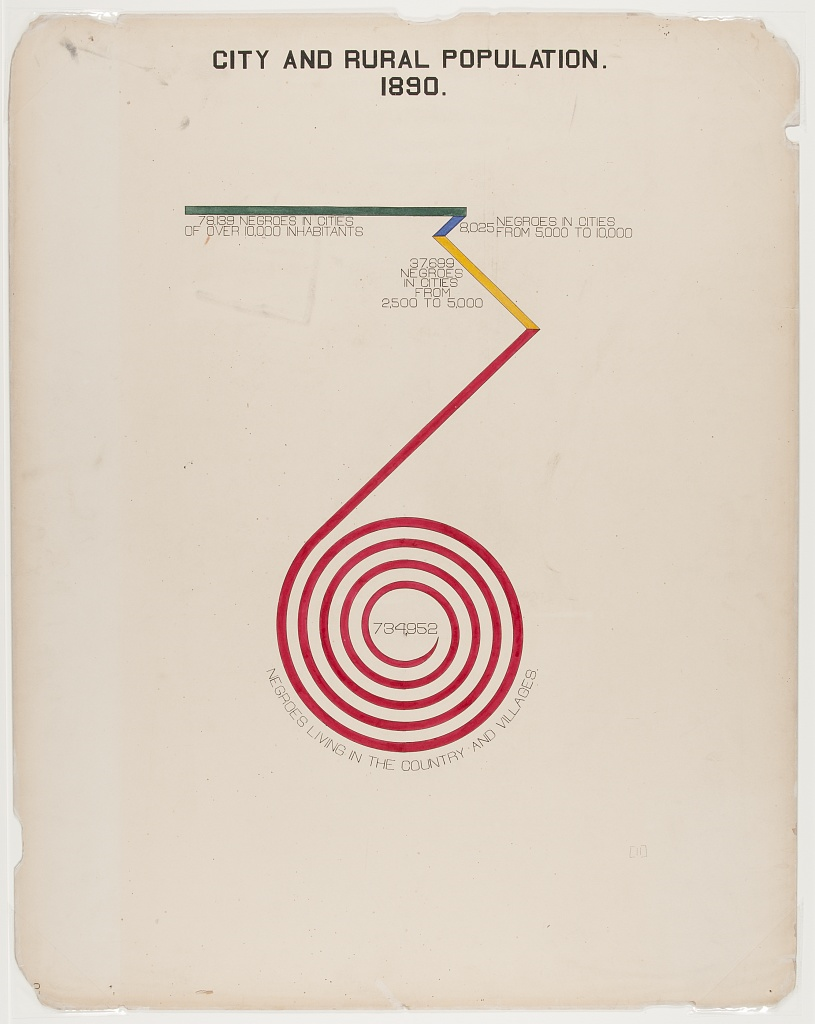
\includegraphics[width=1\textwidth]{figures/intro/du_bois_spinny.png}
        \caption{}
        \label{fig:intro_dpa}
    \end{subfigure}
    \begin{subfigure}{.24\textwidth}
        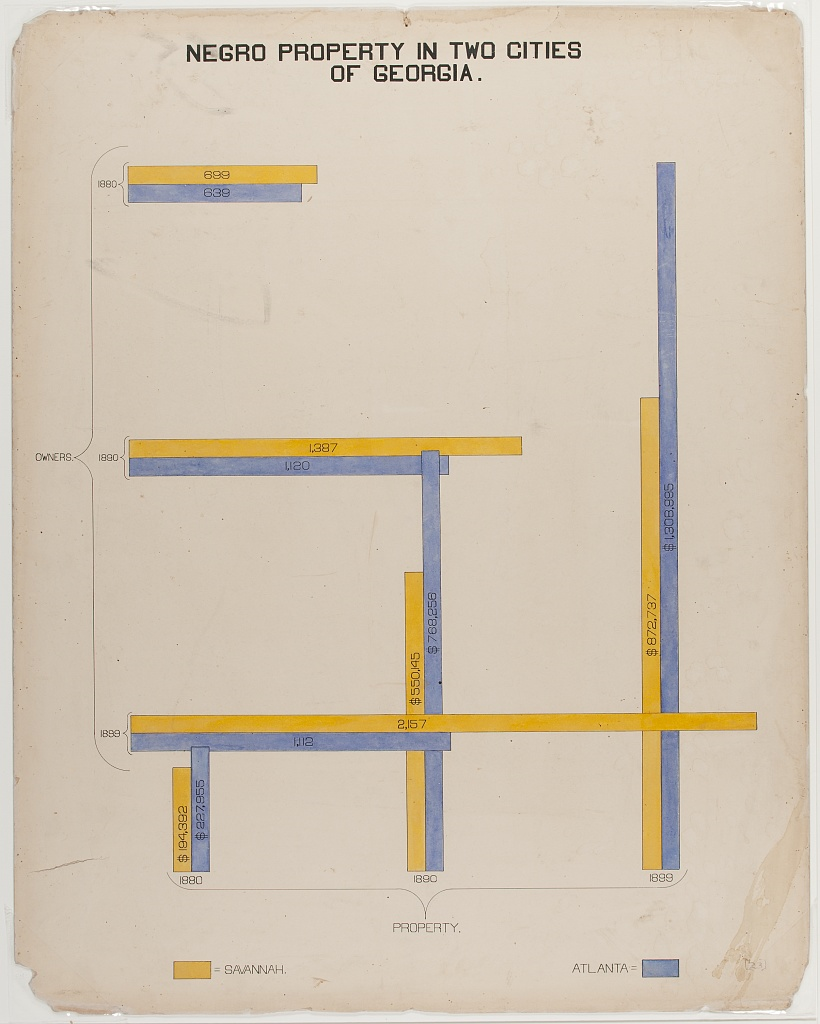
\includegraphics[width=1\textwidth]{figures/intro/du_bois_bar.png}
        \caption{}
        \label{fig:intro_dpb}
    \end{subfigure}
    \begin{subfigure}{.24\textwidth}
        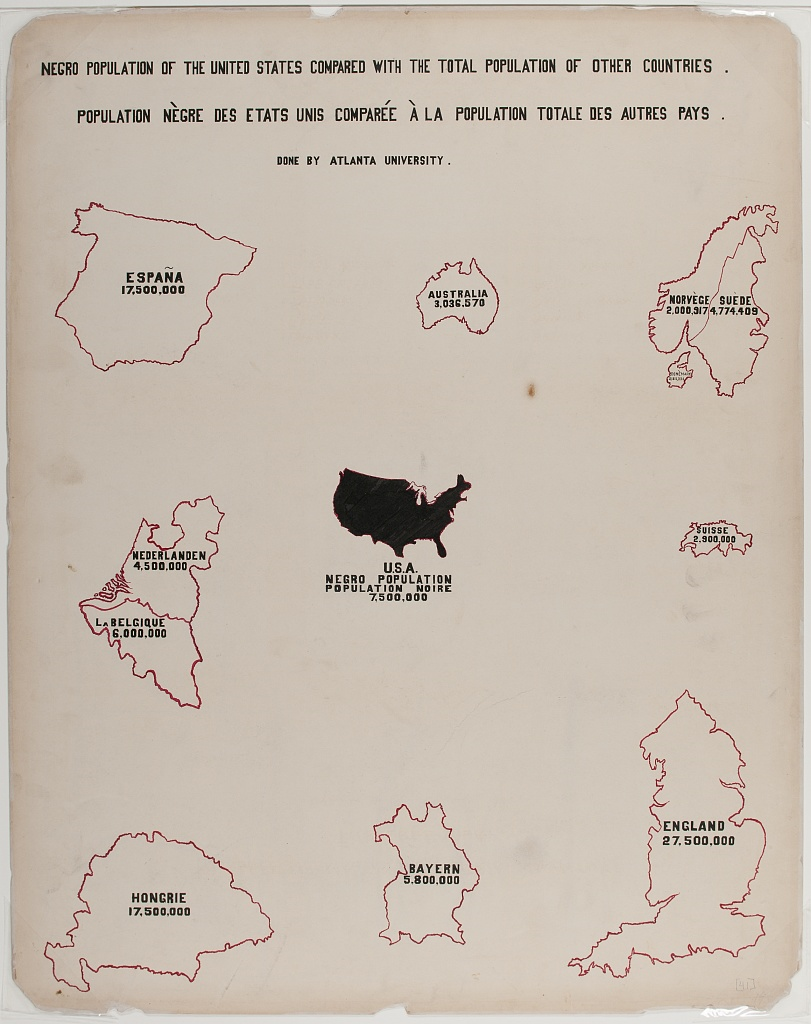
\includegraphics[width=1\textwidth]{figures/intro/du_bois_country.png}
        \caption{}
        \label{fig:intro_dbc}
    \end{subfigure}
    \begin{subfigure}{.24\textwidth}
        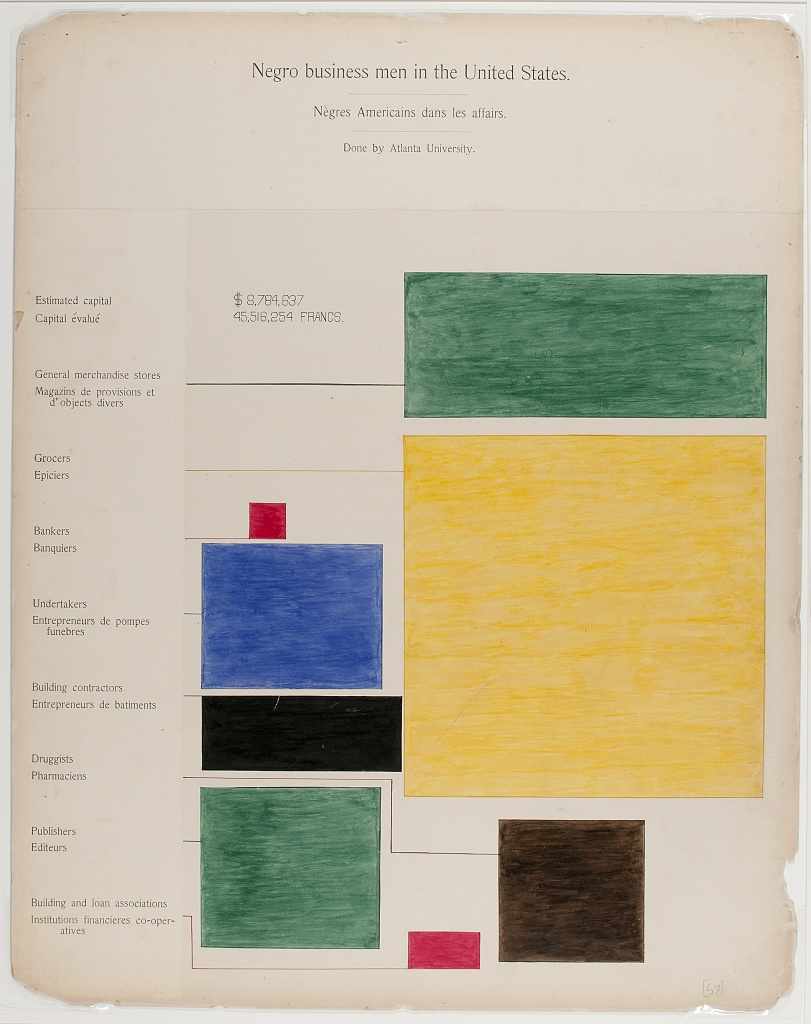
\includegraphics[width=1\textwidth]{figures/intro/du_bois_heat.png}
        \caption{}
        \label{fig:intro_dbd}
    \end{subfigure}
    \caption{Du Bois' data portraits\cite{duboiscenterattheuniversityofmassachusettsBoisDataPortraits2018} of post reconstruction Black American life exemplify that the fundemental characteristics of data visualization is that the visual elements vary in proportion to the source data. In figure~\ref{fig:intro_dpa}, the length of each segment maps to population; in figure~\ref{fig:intro_dpb}, the bar charts are intersected to show the number of property owners and how much they own in a given year; in figure~\ref{fig:intro_dbc} the countries are scaled to population size; and figure~\ref{fig:intro_dbd} is a treemap where the area of the rectangle is representative of the number of businesses in each field. The images here are from the Prints and Photographs collection of the Library of Congress \cite{duboisGeorgiaNegroCity1900,duboisGeorgiaNegroNegro1900, duboisSeriesStatisticalCharts, duboisSeriesStatisticalChartsa}}
    \label{fig:intro_dubois}
\end{figure}

This work aims to develop a model of visualization such that a tool built using this model could support visualizations as varied as those of Du Bois in figure~\ref{fig:intro_dubois}; to do so, we first discuss the criteria by which a visualization is evaluated. Byrne et al. propose that visualizations have graphic representations that are mappings from data to visuals and figurative representations that have meaning due to their similarity in shape to external concepts \cite{byrneAcquiredCodesMeaning2016}. In figure~\ref{fig:intro_dbc}, Du Bois combines a graphical representation where glyph size varies by population with a figurative representation of those glyphs as the countries the data is from, which means that the semantic and numerical properties of the data are preserved in the graph. Tufte specifies that visual representations must be in proportion to the quantitative data being represented for a chart to be faithful and that there should be no extra information in the graphic or figurative elements of the graph, but otherwise his notion of graphic integrity is heavily context dependent\cite{tufteVisualDisplayQuantitative2001}. As is Norman's Naturalness Principal, which states that visualizations are more understandable  when the properties of the representation match the properties of the information being represented\cite{norman_things_smart}. Bertin takes it as a given that data properties match visual properties, so much so that Munzner argues it is inherently built into his classification system \cite{munznerVisualizationAnalysisDesign2014} which is displayed in figure~\ref{fig:intro_retinal_variables}.

\begin{figure}[H]
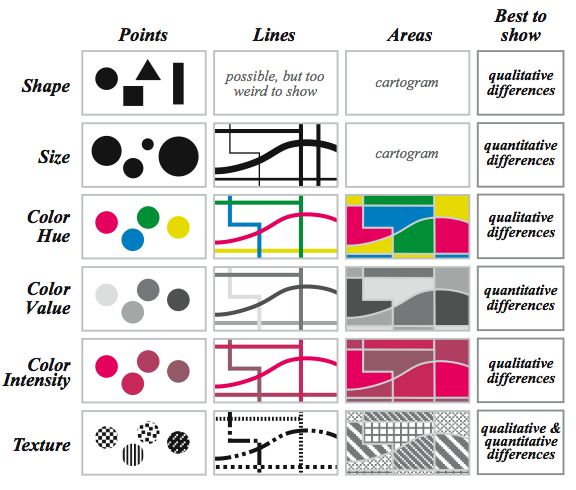
\includegraphics[width=1\textwidth]{figures/intro/retinal_variables.png}
\caption{Retinal variables are a codification of how position, size, shape, color and texture are used to illustrate variations in the components of a visualization. The best to show column describes which types of information can be expressed in the corresponding visual encoding. This tabular form of Bertin's retinal variables is from Understanding Graphics \cite{malamedInformationDisplayTips2010} who reproduced it from \textit{Making Maps: A Visual Guide to Map Design for GIS} 
\cite{krygierMakingMapsVisual2005}}
\label{fig:intro_retinal_variables}
\end{figure}

As described by Mackinlay, a visualization tool produces a graphical design and an image rendered based on that design. He defines the graphical design as the set encoding relations from data to visual representation\cite{mackinlayAutomatingDesignGraphical1986}, and the design rendered in an idealized abstract space is what throughout this paper we will refer to as a graphic. Mackinlay  proposes that a visualization tool's expressiveness is a measure of how much of the structure of the data the tool encodes, while the tools effectiveness describes how much design choices are made in deference to perceptual saliency \cite{clevelandResearchStatisticalGraphics1987,clevelandGraphicalPerceptionTheory1984,chambersGraphicalMethodsData1983a, munznerVisualizationAnalysisDesign2014}. Mackinlay's definition of expressiveness is formalized at the visual encoding level, which as shown in figure~\ref{fig:intro_retinal_variables} refers to the components of a graphic such as the color or position of a glyph. Bertin first classified these graphic components as retinal variables and discussed which types of data they can express \cite{bertinIIPropertiesGraphic2011} and how they are composited on point, line, and area graphical marks, as shown in figure~\ref{fig:intro_retinal_variables} correspond. Marks can be generalized to glyphs, which are graphical objects that convey one or more attributes of the data entity mapped to it\cite{ware2019information, munznerVisualizationAnalysisDesign2014}. 

Mackinlay's expressiveness criteria is well defined for the visual variables, such that he suggests the viability of a strict encoding relation that is a homomorphic mapping which preserves some binary operator from one domain to another \cite{mackinlayAUTOMATICDESIGNGRAPHICAL1987}. We expand on this suggestion by proposing that monoid action equivariance is a strict condition of building valid encoders. Mackinlay does not provide a generalized criteria for plot types, instead embedding the requirements within the definition of the charts. 





\subsection{contribution}
The contribition of this work is 

\begin{enumerate}
    \item functional paradigm visualization tool architecture
    \item translating dataset connectivity into graphical objects via topology-preserving maps
    \item defining transforms from data into graphical components as monoidal action equivariant maps
    \item a model of data and graphics as fiber bundles that decouples components from connectivity
    \item an algebraic sum operation such that more complex visualizations can be built from simple ones 
    \item prototype where we represent the topological base spaces using triangulation, make use of programming types for the fiber, and build on Matplotlib's existing infrastructure for the rendering 
\end{enumerate}
\end{document}